\section{Fluxional execution model} \label{section:model}

% The compiler we present in section \ref{section:compiler} focuses on web applications that tend to follow the functional paradigm while keeping a global memory.
% Such applications are built using functions that are executed sequentially to assure the exclusivity of access on the global memory.
% This is a serious performance issue, as it avoids to leverage the parallelism of modern architectures.

% We present in this section a different execution model that isolates the memory accessible to some functions.
% This approach allows to execute these functions in parallel, hence, to benefit of the performance improvements of this parallelism.
% This execution model is close to the actor model, as the function are executed on autonomous execution units with their own isolated memory, communicating by messages.

% In this section, we present an execution model to allow the execution of functions in parallel of a main thread.
% Each parallel function is encapsulated in an autonomous execution container with its own memory.

This section presents an execution model to provide scalability to web applications with a granularity of parallelism at the function level.
Functions are encapsulated in autonomous execution containers with their state, so as to be mobile and parallel, similarly to the actors model.
And the communications are similar to the dataflow programming model, which allows to reason on the throughput of these streams, and to react to load increases \cite{Bartenstein2014}.
% This execution model is close to the actors model, as the execution containers are independent and communicate by messages.
% As we focus on real-time web applications, the streams of message correspond to the input stream of requests.

% This execution model is also close to the functional paradigm, as the execution container contains function to execute at each message reception.
% The function receives parameters from the input message, and sends one, or more, output streams of messages to other execution container.

The fluxional execution model executes programs written in our high-level fluxionnal language, whose grammar is presented in figure \ref{fig:flx-lang}.
An application $\bnfpn{program}$ is partitioned into parts encapsulated in autonomous execution containers named \textit{fluxions} $\bnfpn{flx}$.
The following paragraphs present the \textit{fluxions} and the messaging system to carry the communications between \textit{fluxions}, and then an example application using this execution model.

\subsection{Fluxions and Messaging System}
% $\bnfpn{flx}$
% $\bnfpn{id}$
% $\bnfpn{fn}$
% $\bnfpn{ctx}$
% $\bnfpn{fn}$
% $\bnfpn{stream}$
% $\bnfpn{dest}$

% The fluxional execution model manages and invokes fluxions.
A \textit{fluxion} $\bnfpn{flx}$ is named by a unique identifier $\bnfpn{id}$ to receive messages, and might be part of one or more groups indicated by tags $\bnfpn{tags}$.
A \textit{fluxion} is composed of a processing function $\bnfpn{fn}$, and a local memory called a \textit{context} $\bnfpn{ctx}$.
% Figure \ref{fig:flx-lang} presents the fluxionnal language we designed to express fluxions.
% The function encapsulated by a \textit{fluxion} consumes an input stream and generates one or more outputs streams.

At a message reception, the \textit{fluxion} modifies its \textit{context}, and sends messages to downstream \textit{fluxions} on its output streams $\bnfpn{streams}$.
The \textit{context} stores the state on which a \textit{fluxion} relies between two message receptions.
% The messaging system carries the stream communications between fluxions based on the names of the recipient fluxions.
% After the execution of a \textit{fluxion},
The messaging system queues the output messages for the event loop to process them later by calling the downstream \textit{fluxions}.
% A message is composed of the recipient fluxions' names and a body.
% Message passing is unable\footnote{at reasonable costs} to replace the synchronization allowed by shared state. % and required between some of the application parts.

In addition to message passing, the execution model allows \textit{fluxions} to communicate by sharing state between their \textit{contexts}.
% To allow this synchronization when required, the execution model allows fluxions to share state between their contexts.
The fluxions that need this synchronization are grouped with the same tag, and loose their independence.
% To assure the consistency of the shared state, all the fluxions of a group are executed sequentially.
% Though, the different groups of fluxions are executed in parallel.

There are two types of streams, \textit{start} and \textit{post}, which correspond to the nature of the rupture point yielding the stream.
A variable created within a chain of \textit{post} streams requires more synchronization than a variable created upstream a \textit{start} stream.
The two types and implications of rupture points are further detailed in section \ref{section:compiler}.
% We differentiate the two types with two different arrows, double arrow (\texttt{>>})                         for \textit{start} rupture points and simple arrow (\texttt{->})          for \textit{post} rupture points.
\textit{Start} rupture points are indicated with double arrow ($\to$ \hspace{-1.4em} $\to$ or \texttt{>>}) and \textit{post} rupture points with simple arrow ($\to$ or \texttt{->}).


% It is the target for our compiler.
\begin{figure}[h]
\vspace{-0.6\baselineskip}
\begin{bnf*}
  \bnfprod{program}    {\bnfpn{flx} \bnfor \bnfpn{flx} \bnfsp \bnftd{eol} \bnfsp \bnfpn{program}}\\
  \bnfprod{flx}        {\bnfts{\texttt{flx}} \bnfsp \bnfpn{id} \bnfsp \bnfpn{tags} \bnfsp \bnfpn{ctx} \bnfsp \bnftd{eol} \bnfsp \bnfpn{streams} \bnfsp \bnftd{eol} \bnfsp \bnfpn{fn}}\\
  % \bnfprod{tags}       {\bnfts{\bnfpn{id}} \bnfor \bnfpn{id} \bnfsp \bnftd{eol} \bnfsp \bnfpn{tags} \bnfor \bnftd{empty string}}\\
  \bnfprod{tags}       {\bnfts{\texttt{\&}} \bnfsp \bnfpn{list} \bnfor \bnftd{empty string}}\\
  \bnfprod{streams}    {\bnfts{\texttt{null}} \bnfor \bnfpn{stream} \bnfor \bnfpn{stream} \bnfsp \bnftd{eol} \bnfsp \bnfpn{streams}}\\
  \bnfprod{stream}     {\bnfpn{type} \bnfsp \bnfpn{dest} \bnfsp [\bnfpn{msg}]}\\
  \bnfprod{dest}       {\bnfpn{list}}\\
  \bnfprod{ctx}        {\bnfts{\texttt{\{}} \bnfpn{list} \bnfts{\texttt{\}}}}\\
  \bnfprod{msg}        {\bnfts{\texttt{[}} \bnfpn{list} \bnfts{\texttt{]}}}\\
  \bnfprod{list}       {\bnfpn{id} \bnfor \bnfpn{id} \bnfsp \bnfts{,} \bnfsp \bnfpn{list}}\\
  \bnfprod{type}       {\bnfts{\texttt{>}\texttt{>}} \bnfor \bnfts{\texttt{-}\texttt{>}}}\\
  \bnfprod{id}         {\bnftd{Identifier}}\\
  \bnfprod{fn}         {\bnftd{Source language with~} \bnfpn{stream} \bnftd{~placeholders}}\\
\end{bnf*}
\vspace{-2.5\baselineskip}
\caption{Syntax of a high-level language to represent a program in the fluxionnal form}
\label{fig:flx-lang}
\end{figure}

% Fluxions are executed on an event-loop with an isolated heap ; it is a \textit{Node.js} instance.
% We propose to stretch the execution of an application by distributing the fluxions on different event-loops.
% But the distribution is limited by the dependencies between fluxions.
% All the fluxions of a group need to be gathered on the same event-loop.
% Indeed, each event-loop assures the exclusivity of access to the state: only one fluxion is executed at once.
% Consequently, the more fluxions are gathered on an event-loop, the less time fraction each fluxion can use without impacting the throughput.

%These groups represent the graph of state communications between fluxion.
%Hence, this graph indicates the states that are limiting the parallelism.


% A fluxion receiving and sending heap reference can be stateless, hence replicated.
% However, because it share references, it needs to be on the same group than other another fluxions (think about req / res).
% If all the fluxion of a group are stateless, they can be replicated exactly like if it was a single fluxion. 





% \subsection{Messaging system}

% In a distributed approach, the messages between fluxions would be carried over a distributed message broker.
% However this execution model is only a simulation of a distributed execution environement.
% We simplify the distributed message broker with a master message queue to centralize communication between workers, though, each worker has its own local message queue.
% The messaging system is the core of the execution model.
% It carries messages and invokes fluxions at reception.
% The messaging system sends messages to the worker hosting the destination fluxion.
% Locally, the master worker hosts fluxions that need access to the external network or the global memory.
% Using a message queue allows to execute multiple processing chains fairly and concurrently, without difference in scheduling local messages, or network messages.

% The messages are queued for the event-loop to execute the associated fluxions sequentially.

% The execution model allows each group of fluxions to be executed on a remote event-loop.
% Therefore, some messages need to be send to remote event-loops.
% When processing a message, if the destination fluxion is local, the messaging system immediately invokes the fluxion with the message, if it is on a remote event-loop, the messaging system sends the message to be queued on the remote event-loop.



% The messaging system carries messages from one event-loop to the other, and assure that the message is queued on the event-loop executing the destination fluxion.

% If two fluxions share the same name, it would lead to a conflicting situation for the messaging system.

% This registration associates a processing function with a unique name and an initial \textit{context}.
% The registration is done by calling \texttt{register(<name>, <fn>, <context>)}, \circled{1}.
% A fluxion can dynamically register other fluxions

% \nt{the example in figure 2 is only partially explained in text, many parts (group network, program, enqueue...) are not explained.}

% Algorithms \ref{alg:parcours} and \ref{alg:traitement} describe the behavior of the messaging system after the \texttt{start} function invocation.

% \begin{algorithm}
% \caption{Message queue walking algorithm}
% \label{alg:parcours}
% \begin{algorithmic}
% \Function{loopMessage}{\null}
% \While{$msg$ \textbf{presents in} $msgQueue$}
% \State $msg \gets$ \Call{dequeue}{\null} \Comment{\circled{3}}
% \State \Call{ProcessMsg}{$msg$}
% \EndWhile
% \EndFunction
% \end{algorithmic}
% \end{algorithm}

% \begin{algorithm}
% \caption{Message processing algorithm}
% \label{alg:traitement}
% \begin{algorithmic}
% \Function{processMsg}{$msg$}
% \For{$dest$ \textbf{in} $msg.dest$}
% \State $worker \gets lookup(dest)$
% \State \Call{worker.send}{$fluxion, msg.body$} \Comment{\circled{4}}
% % \State $message \gets$ \Call{exec}{$fluxion, msg.body$} \Comment{\circled{4} \& \circled{5}}
% % \State \Call{enqueue}{$message$} \Comment{\circled{6}}
% \EndFor
% \EndFunction
% \end{algorithmic}
% \end{algorithm}

\subsection{Example}

\begin{code}[js,
  caption={Example web application},
  label={lst:source}]
var app = require('express')(),
    fs = require('fs'),
    count = 0; //@\label{lst:source-counter}@

app.get('/', function handler(req, res){ //@\label{lst:source-handler}@
  fs.readFile(__filename, function reply(err, data) {
    count += 1;
    res.send(err || template(count, data)); //@\label{lst:source-send}@
  });
}); //@\label{lst:source-handler-end}@

app.listen(8080);
\end{code}

The fluxional execution model is illustrated with an example application presented in listing \ref{lst:source}.
This application reads a file, and sends it back along with a request counter.
The \texttt{handler} function, line \ref{lst:source-handler} to \ref{lst:source-handler-end}, receives the input stream of requests.
The \texttt{count} variable at line \ref{lst:source-counter} counts the requests, and needs to be persisted between two messages receptions.% in the fluxion \textit{context}.
The \texttt{template} function formats the output stream to be sent back to the client.
The \texttt{app.get} and \texttt{res.send} functions, lines \ref{lst:source-handler} and \ref{lst:source-send}, interface the application with the clients.
And between these two interface functions is a chain of three functions to process the client requests : \texttt{app.get} $\to$ \hspace{-1.4em} $\to$ \texttt{handler} $\to$ \texttt{reply}.
This chain of functions is transformed into a pipeline, expressed in the high-level fluxionnal language in listing \ref{lst:fluxional}.
The transformation pocess between the source and the fluxional code is explained later, in section \ref{section:compiler}.

\begin{figure}[h!]
  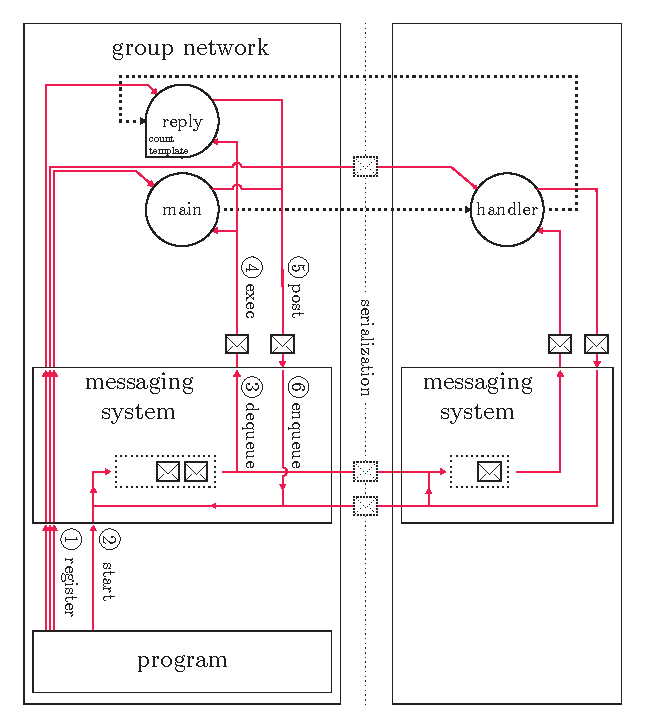
\includegraphics[width=\linewidth]{ressources/schema-message.pdf}
  \caption{The fluxionnal execution model in details}
  \label{fig:MesSys}
\end{figure}

The execution is illsutrated in figure \ref{fig:MesSys}.
The dashed arrows between fluxions represent the message streams as seen in the fluxionnal application.
The plain arrows represent the operations of the messaging system during the execution.
These steps are indicated by numeroted circles.
% In the execution cycle of the example, illustrated in figure \ref{fig:MesSys}, numeroted circles indicate the step in the execution.
% The bigger circles represent the registered fluxions.
The \textit{program} register the fluxions in the messageing system, \circled{1}.
The fluxion \textit{reply} has a context containing the variable \texttt{count} and \texttt{tem\-plate}.
% The streams between workers are serialized.
% To assure the consistency of their shared contexts, all the fluxions grouped with the same tag are executed sequentially and share the same message queue.
% Though, the different groups of fluxions are executed in parallel with different event queues.
% This first message represents the incoming of a request from a user.
When the application receives a request, the first fluxion in the stream, \textit{main}, queues a \texttt{start} message containing the request, \circled{2}.
This first message is to be received by the next fluxion \textit{handler}, \circled{3}, and triggers its execution, \circled{4}.
The fluxion \textit{handler} sends back a message, \circled{5}, to be enqueued, \circled{6}.
The system loops through steps \circled{3} through \circled{6} until the queue is empty.
This cycle starts again for each new incoming request causing another \texttt{start} message.

% The original source code of this application is available in listing \ref{lst:source}\footnote{The listings are also available on github\cite{flx-example}.}.
% In this example application, some points are worth noticing.

% We expect a similar result with the compiler described in section \ref{section:compiler}.
% Horizontal dashed lines show virtual transmission of messages between fluxions although they all go through the messaging system.

% \begin{figure}[h!]
%   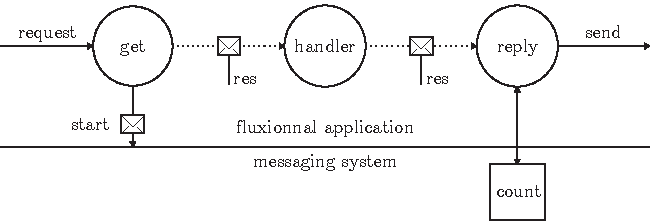
\includegraphics[width=\linewidth]{ressources/flux.pdf}
%   \caption{Fluxions chain manually extracted from the example application}
%   \label{fig:fluxions}
% \end{figure}

\begin{code}[flx, caption={Example application expressed in the high-level fluxional language}, label={lst:fluxional}]
flx main & grp_res
>> handler [res]
  var app = require('express')(),
      fs = require('fs'),
      count = 0;

  app.get('/', >> handler); //@\label{lst:fluxional-streamtohandler}@
  app.listen(8080);

flx handler
-> reply [res]
  function handler(req, res) {
    fs.readFile(__filename, -> reply); //@\label{lst:fluxional-readfile}@
  }

flx reply & grp_res {count, template}
-> null
  function reply(error, data) {
    count += 1; //@\label{lst:fluxional-counter}@
    res.send(err || template(count, data)); //@\label{lst:fluxional-ressend}@
  }
\end{code}

% The application is organized as follow.
The chain of functions from listing \ref{lst:source} is expressed in the fluxional language in listing \ref{lst:fluxional}.
% The stream of requests is received from the clients by the fluxion \texttt{main}, it continues in the fluxion \texttt{handler}, and finally goes through the fluxion \texttt{reply} to be sent back to the clients.
The fluxion \texttt{handler} doesn't have any dependencies, so it can be executed in a parallel event-loop.
The fluxions \texttt{main} and \texttt{reply} belong to the group \texttt{grp\_res}, indicating their dependency over the variable \texttt{res}.
The group name is arbitrarily chosen by the compiler.
% The last fluxion, \texttt{reply}, depends on the variable \texttt{res} created by the first fluxion, \texttt{main}.
% This variable is carried by the stream through the chain of fluxion to the fluxion \texttt{reply} that depends on it.
% The group \texttt{network} depends on this variable because it holds the references to the network sockets.
All the fluxions inside a group are executed sequentially on the same event-loop, to protect against concurrent accesses.

The variable \texttt{res} is created and consumed within a chain of \textit{post} stream.
Therefore, it is exclusive to one request and cannot be propagated to another request.
It doesn't prevent the whole group from being replicated.
However, the fluxion \texttt{reply} depends on the variable \texttt{count} created upstream the \textit{start} stream, which prevents this replication.
If it did not rely on this state, the group \texttt{grp\_res} would be stateless, and could be replicated to cope with the incoming traffic.

This execution model allows to parallelize the execution of an application as a pipeline, like with the fluxion \texttt{handler}.
And some parts are replicated, as could be the group \texttt{grp\_res}.
This parallelization improves the scalability of the application.
Indeed, as a fluxion contains its state and expresses its dependencies, it can be migrated.
It allows to adapt the number of fluxions per core to adjust the resource usage in function of the desired throughput.

Our goal, as described in the introduction, is not to propose a new high-level language but to automate the architecture shift.
We present the compiler to automate this architecture shift in the next section.

\nt{I would also suggest adding labels to one of the fluxions in listing 2 to indicate its tags, context, steams and function.}
